% !TeX root = tutorial1.tex
\documentclass[12pt,letterpaper]{article}
% Packages go before \begin{document} but after \documentclass
\usepackage[margin=1in]{geometry} % Set Margins to 1 inch standard
\usepackage{amsmath} % Package for math equations.
\usepackage{graphicx} % Package for Embedded Figures

\begin{document}
\title{Joel's \LaTeX\ Tutorial}
\author{Joel M. Brigida: ADolbyB}
\maketitle % Document Title

\pagebreak

\tableofcontents

\pagebreak

\section{First Section: Description and Figures}

This is a \LaTeX\ Tutorial. In this tutorial I am going to embed a bunch of different stuff. What happens now?
I'll circle back to this part after I'm done doing other stuff.

\medskip

\begin{figure}[h!] % [h!] for here! to place figure on 1st page. Otherwise its on 2nd Page
    \center
    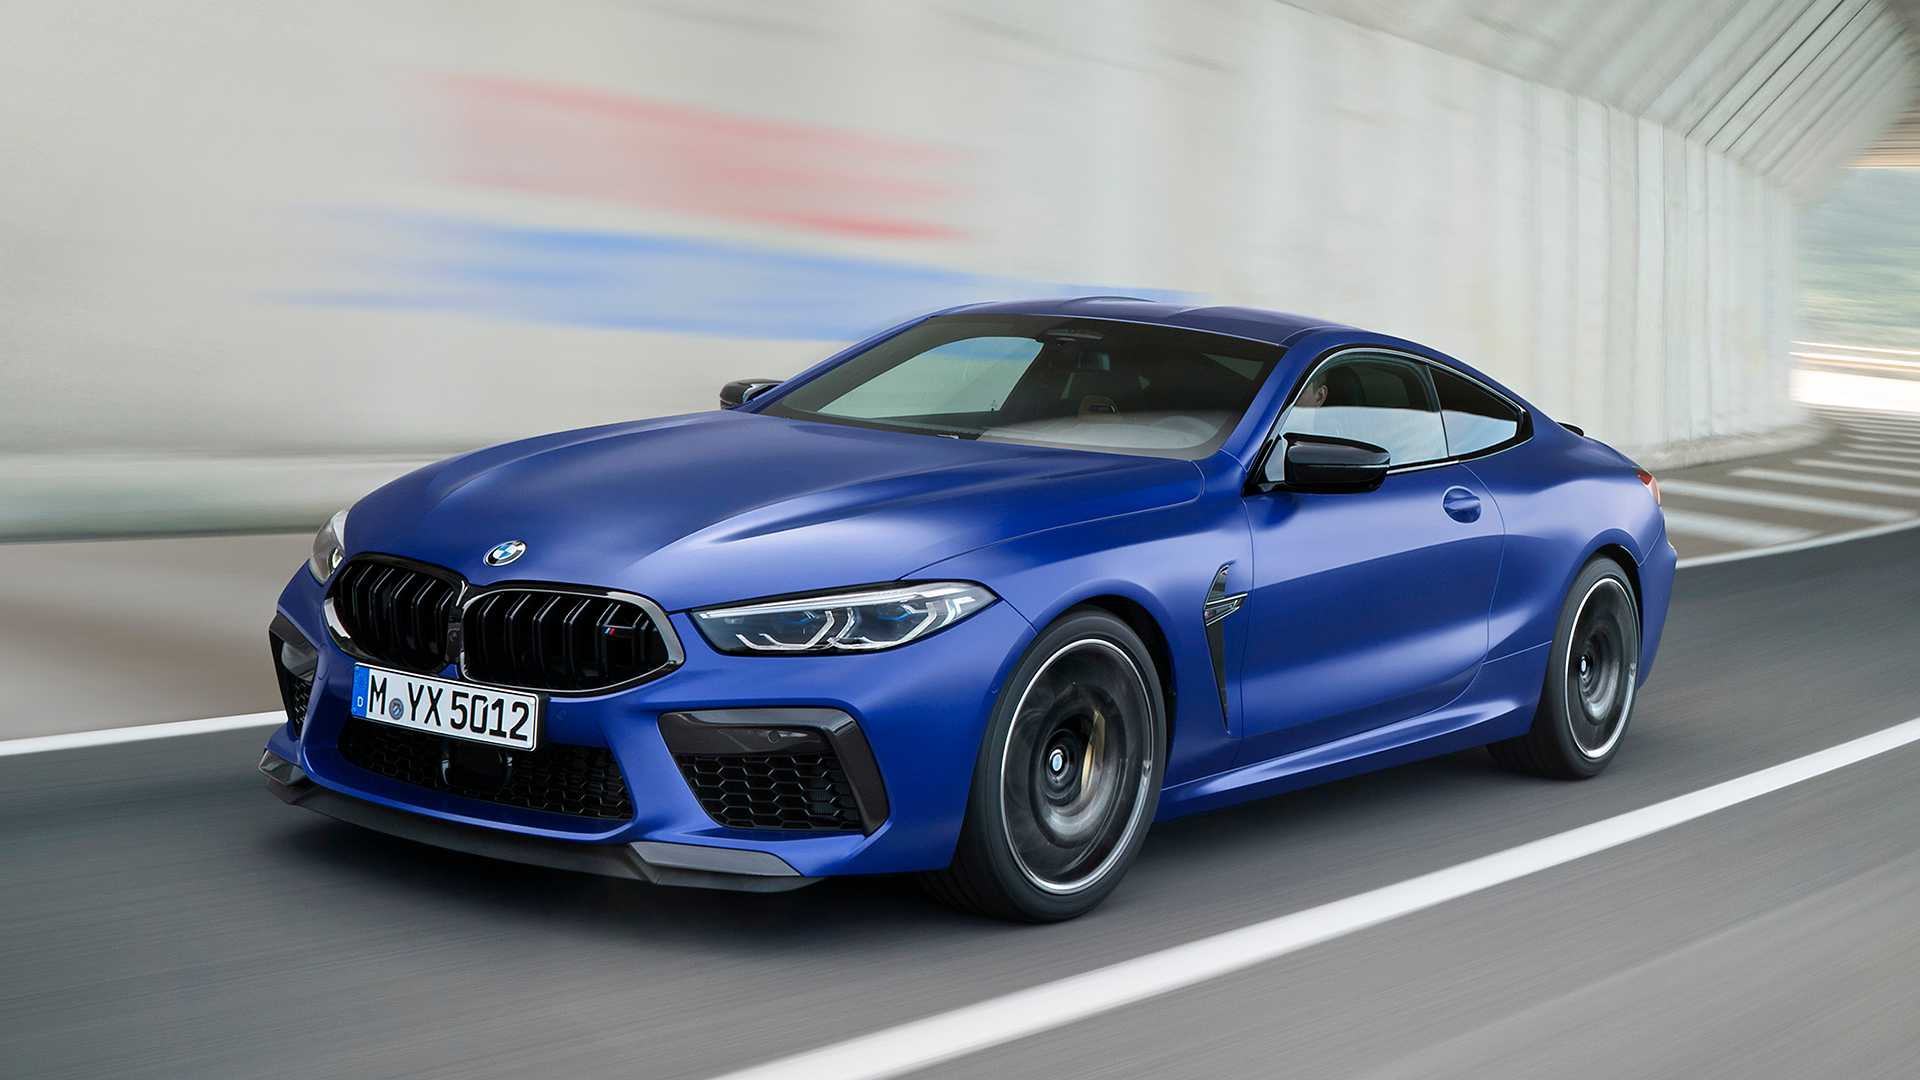
\includegraphics[width=\linewidth]{2019m8.jpg}
    \caption{2019 BMW M8 Coupe}
\end{figure}

\pagebreak

\section{Second Section: Math Equations}

The Equation for a Straight Line is:
\begin{equation}
    y = mx + b
\end{equation}

The Quadratic Equation is:

\begin{equation}
    x = \frac{-b \pm \sqrt{b^2 - 4ac}}{2a}
\end{equation}
\medskip

The Theory of Special Relativity is:

\begin{equation}
    e = mc^2
\end{equation}

\section{Third Section: Simple Tables}

\begin{table}[h!]
    \caption{This Is A Simple Table}
    \begin{center}
        \begin{tabular}{c c c} % number of columns = 2: 'c c'
            $x$ & $y$ &  $z$\\
            \hline
            6 & 9 & 42\\
            \hline
            46 & 2 & 41\\
        \end{tabular}
    \end{center}
\end{table}

\end{document}